\chapter{The LHCb detector at the Large Hadron Collider}
\label{sec:Detector}

\section{The Large Hadron Collider}

The Large Hadron Collider (LHC) is a circular particle accelerator with a circumference of 27 km about 100 m underground.
The two general-purpose detectors, ATLAS and CMS, sit on opposites sides of the ring, while the two smaller specialty detectors, 
ALICE and LHCb, are at the interaction points to either side of ATLAS (see fig. \ref{lhc}).

\begin{figure}[h!]
\centering
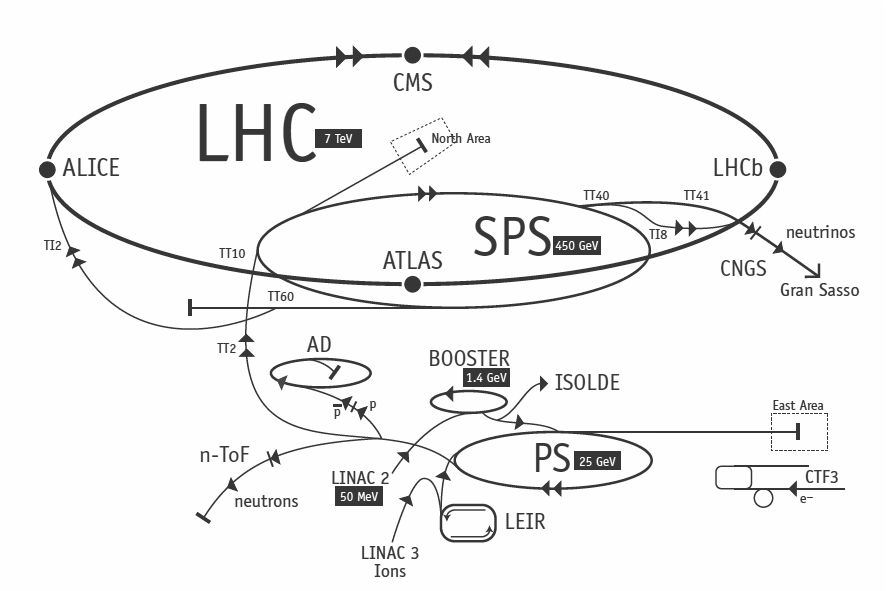
\includegraphics[width=1\textwidth]{Detector/figs/LHC_scheme.png}
\caption{Scheme of CERN accelerators.} \label{lhc}
\end{figure}

Two proton beams circulate in opposite directions around the ring and cross each other at several points, 
in which are placed huge particle detectors. Each beam consists of a series of proton bunches, up to a maximum of 2835
in the beam. Each bunch consists of about $10^{11}$ protons and the bunch spacing is such that the nominal bunch crossing
rate is 40 MHz. The beams are injected into pre-accelerators and then led into LHC through the CERN acceleration
system shown in figure \ref{lhc}. Protons are produced from duoplasmatron, starting from hydrogen gas, and are
initially accelerated to the energy of 50 MeV in a linear accelerator (LINAC). Then, protons are injected into
the Proton Synchrotron Booster (PSB) where they are boosted to an energy of 1.4 \gev, then into the Proton Synchrotron (PS)
to 25 GeV and Super Proton Synchrotron (SPS) to 450 GeV. Finally, protons enter into the LHC storage ring.
In the main ring proton beams are accelerated from injection energy to the final one by radio frequency (RF) cavities.
The beams are steered around the ring by 8 T magnetic fields produced in 15 meter long superconducting niobium-titanium
dipole magnets, and focused by quadrupole and multipole magnets. The LHC magnets use a design in which both proton beam
pipes are contained in the same housing, allowing the same liquid helium to cool the system down for both \cite{lhc}.
The LHC began colliding proton beams in physics mode in 2009 at and energy of $\sqrt{s} = 900$ GeV and from April 2010
to November 2011 accelerated beams at $\sqrt{s} = 7$ TeV (3.5 TeV per proton beam). At this energy it delivered over
$5.7 \text{ fb}^{-1}$ of collisions, with a maximum instantaneous luminosity of $3\cdot10^{33} \text{ cm}^{-2}\text{s}^{-1}$.
The LHC maximum design energy is 14 TeV, and its design luminosity is $10^{34} \text{ cm}^{-2}\text{s}^{-1}$.
After a long shut down to upgrade and maintain the machine, a new run started in June 2015 where protons
are collided at an energy of $\sqrt{s} = 13$ \tev at this energy the total proton-proton cross section
is expected to be roughly 100 mb.
%, thus at the design luminosity the general purpose detectors will an event rate approximately $10^9$ inelastic events/s.

\section{The LHCb detector}

The LHCb detector was built with the main purpose of studying the decays of B and D mesons, looking in particular for CP-violating processes. In 2011, running at a centre of mass energy of 7 TeV, the cross section of $b\bar{b}$ production was measured to be $284 \pm 53 ~\mu b$\cite{Aaij:2010gn}, while it will be $\sim500 ~\mu b$ at the nominal LHC energy, 14 TeV.
At these high energies, proton-proton interactions produce highly boosted virtual gluons which interact to produce $b\bar{b}$ pairs at small angles, close to the beam pipe. For this reason the LHCb detector is designed to have a very forward angular coverage: it is fully instrumented from approximately 10 mrad to 300 mrad, corresponding to $2 < \eta < 5$, where $\eta$ is a quantity used in particle physics and called ``pseudorapidity" and defined as:
\begin{equation}
\label{pseudorap}
\eta = - \ln(\tan(\theta/2))
\end{equation}
In Eq. \ref{pseudorap}, $\theta$ is the angle between a particle's momentum and the beam direction\footnote{LHCb's reference system has the $z$ axis in the direction of the beam, the $x$ axis directed to the centre of the accelerator and $y$ is directed upward. Then we define $\theta$ as the angle with the beam direction and $\phi$ as the position around the beam in the $xy$ plane, taking $\phi = 0$ on the $x$ axis.}.

\begin{figure}[h]
\label{lhcb}
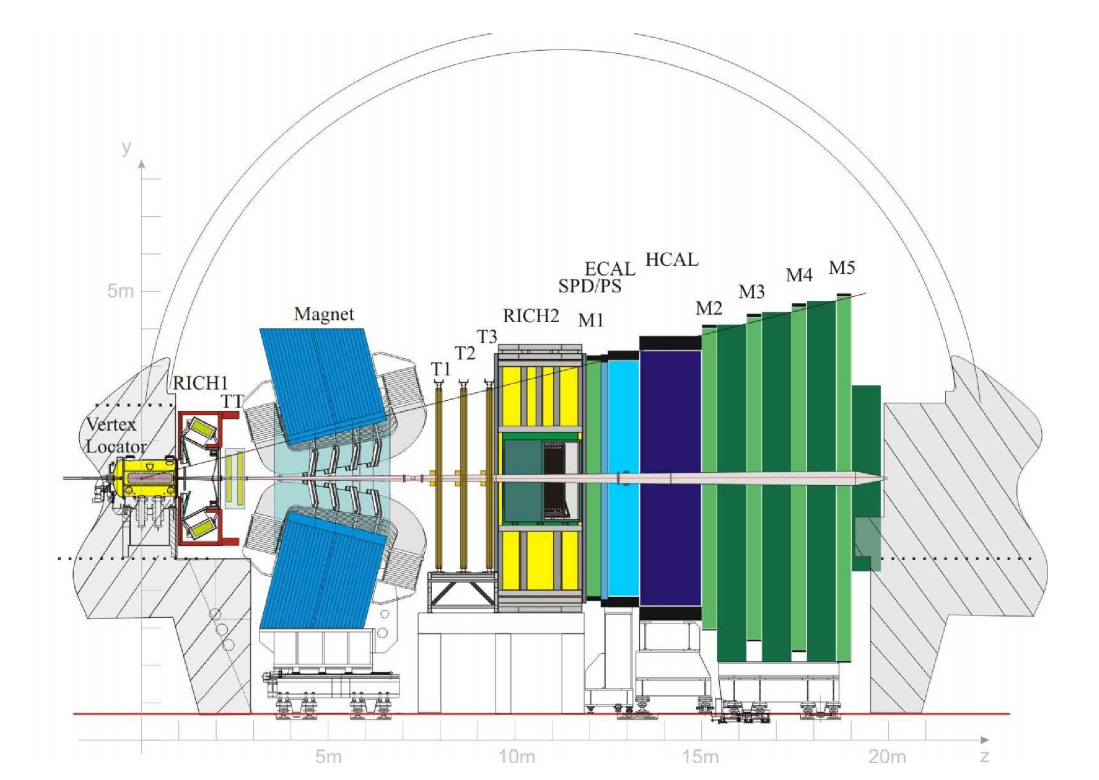
\includegraphics[width=0.9\linewidth]{Detector/figs/LHCb_official.png}
\caption{A side view of the LHCb detector \cite{Alves:2008zz}.}
\end{figure}

At the collision point of LHCb the luminosity can be adjusted by displacing the beams from head on collisions while keeping the same
crossing angle. This allows the experiment to keep an approximately constant instantaneous luminosity. This also means that the average number of interactions per bunch crossing can be limited as LHCb efficiency, especially of detecting secondary vertices, decreases for events with an high number of primary vertices (PV). Reducing the particle occupancy through the detector also keeps radiation damage to a minimum. Since the LHC started colliding protons in
November 2009 until the end of 2011, the instantaneous luminosity was at an average of $3 \cdot 10^{32} \mbox{cm}^{-2}\mbox{s}^{-1}$, with an average number of 1.5 vertices per bunch crossing in LHCb. At the end of 2011 LHCb had collected an integrated luminosity of $1 ~\mbox{fb}^{-1}$; in 2012 the luminosity was increased and $2 ~\mbox{fb}^{-1}$ more were collected.

Other B physics experiments, like BaBar at the Stanford Linear Accelerator (SLAC), Belle at KEK at J-PARC (Japan) and the Tevatron experiments at Fermilab have made accurate measurements in heavy flavour physics. All of these results have so far been consistent with the Standard Model predictions. However, some of the deviations from the Standard Model are expected to be very small, therefore LHCb has begun to make the most precise measurements in heavy flavour physics.

The LHCb detector\cite{Alves:2008zz} includes a high-precision tracking system consisting of a silicon-strip vertex detector surrounding the $pp$ interaction region, a large-area silicon-strip detector located upstream of a dipole magnet with a bending power of about 4 Tm, and three stations of silicon-strip detectors and straw drift tubes placed downstream. The combined tracking system has momentum resolution $\Delta p/p$, that varies from 0.4\% at 5 $\mbox{GeV/c}^{2}$ to 0.6\% at 100 $\mbox{GeV/c}^{2}$.
Charged hadrons are identified using two Ring-Imaging Cherenkov detectors (RICH)\cite{LHCb-DP-2012-003}. Photon, electron and hadron candidates are identified by a calorimeter system consisting of scintillating-pad and pre-shower detectors, an electromagnetic calorimeter and a hadronic calorimeter. Muons are identified by a system composed of alternating layers of iron and multiwire proportional chambers\cite{LHCb-DP-2012-002}. A schematic view of the detector is shown in Fig. \ref{lhcb}.


\subsection{Tracking system}

The tracking system is made up of the Vertex Locator (VeLo), and 4 tracking stations: the Tracker Turicensis (TT) which are located before the magnet and T1, T2 and T3 which are downstream of the magnet. Charged particle tracks are bent horizontally in the magnetic field so that their momentum can be measured from the curvature radius.

B mesons have lifetimes of approximately 1.5 ps. At the LHC energies, this means they travel about 1 cm before decaying and they form a displaced vertex. It is therefore important to be able to separate the particles produced at the primary $p-p$ vertex and the B decay vertex.

The VeLo accurately measures positions of tracks close to the interaction point so that production and decay vertices of bottom and charm hadrons can be reconstructed. The VeLo is made up of 21 staggered silicon modules which surround the beam axis and are positioned from $z = -18$ cm to $+80$ cm. It is able to detect particles within a pseudorapidity range $1.6 < \eta < 4.9$. The sensitive region of the VeLo starts at an inner diameter of 8mm from the beam axis. The VeLo is housed in its own vacuum vessel of thin aluminium foil which protects the vacuum of the beam pipe from any outgassing of the VeLo. VeLo stations consist of two modules, and each has two types of sensors: the $\phi$-sensor which measures the azimuthal position around the beam, and the R-sensor which measures the radial distance from the beam axis. A sketch of the VeLo sensor is shown in Fig. \ref{VeLo}. The sensors are 300 $\mu m$ thick, approximately semicircular and are positioned on either side of the beam axis. To ensure that they cover the full azimuthal angle the right-side module is placed 1.5 cm behind the left-side module on the z-axis and they overlap. There are two modules which cover the backward direction and were used as a veto for multiple interactions in 2011, called the pileup veto.

\begin{center}
\begin{figure}[h!]
\label{VeLo}

\begin{minipage}{0.49\textwidth}

\centering 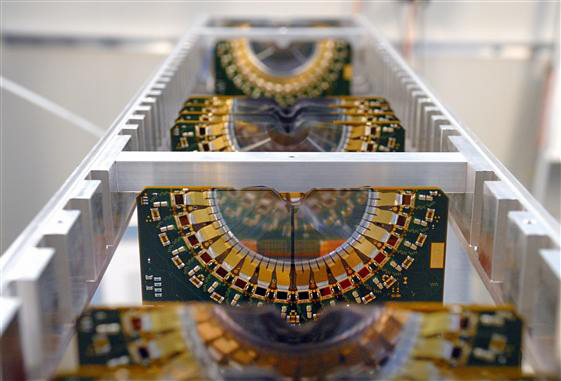
\includegraphics[width=0.8\textwidth]{Detector/figs/detector/VELO.png}

\end{minipage}
\begin{minipage}{0.49\textwidth}

\centering 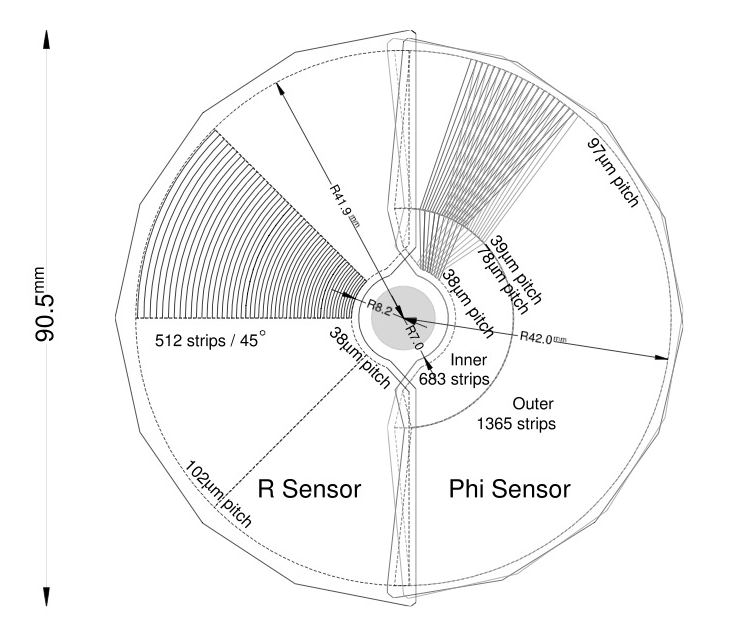
\includegraphics[width=0.8\textwidth]{Detector/figs/detector/VELO_scheme.png}

\end{minipage}
\caption{On the left VeLo sensors mounted in line and on the right a schematic view of one sensor \cite{Alves:2008zz}.}
\end{figure}
\end{center}

The LHCb dipole magnet is comprised of two coils supported on an iron yoke and is wedge-shaped to fit the LHCb 
angular acceptance. It is a warm magnet so can be ramped easily and the field can be reversed periodically. 
This is used to limit some systematics that can arise form imperfections performance in different areas of the detector.

The IT and TT both use silicon microstrip and together constitute the Silicon Tracker (ST). Straw tubes are used 
in the outer regions of the tracking stations which together are called the Outer Tracker (OT). The IT has 
an higher inner granularity because of the higher flux of particles nearer the beam pipe. Each ST station 
has four detection layers, the first and last being vertical, measuring the track position in x. The second 
and third layer are rotated by a stereo angle of +5 and -5 degrees, which allows the y-coordinate to be measured. 
The TT is placed upstream of the magnet which allows reconstruction of the tracks from low-momentum particles which 
are swept out of the downstream acceptance.

\subsection{Particle identification}

Particle identification in LHCb is performed in various ways. The calorimeter detects particles with high 
transverse momentum, the muon chambers identify muons and the Ring Imaging Cherenkov (RICH) detectors identify 
heavier charged particles.

\subsubsection{Calorimeters}
\label{sec:calorimeters}

The main purpose of the calorimeter system is to determine the energy of particles traversing the detector. 
The material in the calorimeter system is layered with absorber and active material. The absorber makes particles
interact and produces a cascade of secondaries, which multiply quickly and are detected by the active part. 
The sensitive material consists of scintillating layers, where the light detected is approximately proportional 
to the number of deposited particles. Calibration is then used to calculate the deposited energy. The calorimeter 
system is essential for flavour tagging because it identifies electrons. In addition, it is required for accurately 
reconstructing
$\pi^0$ particles and prompt photons, which are both needed for the study of B-meson decays. The LHCb calorimeter 
system consists of the Scintillator Pad Detector (SPD), the Pre-Shower Detector (PS) as well as the Electromagnetic 
Calorimeter (ECAL) and the Hadronic Calorimeter (HCAL). All four detectors transmit scintillation light via 
wavelength-shifting fibres to photo-multiplier tubes (PMTs). The SPD/PS cells are read out with MAPMTs 
(Multi-anode PMTs) located outside the LHCb acceptance. The ECAL and HCAL have individual MAPMTs located on the modules.
All four detectors vary the segmentation of their cells according to the distance from the beam pipe.
The purpose of the SPD and PS is to separate the electrons from a high background of neutral and charged pions 
produced in the collisions. In order to obtain the highest energy resolution the showers from high energy photons 
must be fully absorbed. For this reason the ECAL has a thickness of 25 radiation lengths and its resolution is 
measured to be \cite{Alves:2008zz}
 
 \begin{equation}
 \frac{\sigma_{ECAL}(E)}{E} = \frac{10\%}{\sqrt{E(GeV)}} + 1\%
 \end{equation}

The trigger requirements on the HCAL resolution do not depend on the containment of the hadron showers as much 
as for the ECAL, so due to a limited space, its thickness is only 5.6 interaction lengths and its resolution

 \begin{equation}
 \frac{\sigma_{HCAL}(E)}{E} = \frac{69\%}{\sqrt{E(GeV)}} + 9\%
 \end{equation}




\subsubsection{RICH}

The two RICH detectors are a special feature of LHCb, as it is the only experiment at LHC including them. 
These detectors take advantage of the  Cherenkov light produced by particles passing in a medium with velocity 
higher that the velocity of light in the medium. The Cherenkov light, as shown in Fig. \ref{Cherenkov}, 
is produced in cones with a specific angle depending on the velocity of the particle

\begin{equation}
cos(\theta) = \frac{1}{\beta n}
\end{equation}

where $\beta$ is the velocity of the particle over $c$ and $n$ is the refraction index of the medium.

\begin{center}
\begin{figure}[h!]
\label{Cherenkov}

\begin{minipage}{0.45\textwidth}

\centering 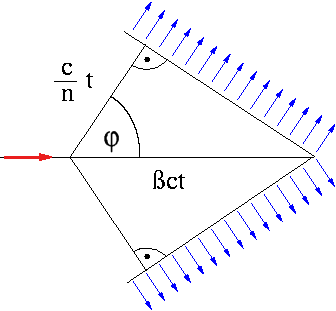
\includegraphics[width=0.8\textwidth]{Detector/figs/detector/Cherenkov.png}

\end{minipage}
\begin{minipage}{0.55\textwidth}

\centering 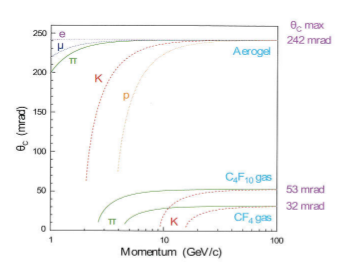
\includegraphics[width=0.8\textwidth]{Detector/figs/detector/RICH_performance.png}

\end{minipage}
\caption{On the left a sketch of Cherenkov light emission \cite{wikiCherenkov} and on the right the Cherenkov
angle versus momentum for the two radiators of RICH1 and for different particles. One can see that they allow
to separate particles in different momentum ranges.}
\end{figure}
\end{center}

RICH 1 is situated before the magnet in order to cover a large angular acceptance. Its purpose is to ensure
particle identification over the momentum range $1 < p < 70$ GeV. It uses two radiators, $C_4F_{10}$ covers
the momentum range $5 - 70$ GeV/c, and silica aerogel which covers $1 - 10$ GeV/c. RICH 2 is situated after
the magnet and tracking stations. It identifies higher momentum particles from approximately 20 GeV up to beyond
100 GeV using $CF_4$ as a radiator.
The Cherenkov light produced when charged particles travel through the radiators, is reflected and focused using
flat and spherical mirrors which are tilted so that the ring image is reflected onto arrays of photo-detectors.
The radius of the ring becomes equivalent to the opening angle of the Cherenkov cone because of the known geometry.
The photo-detectors are located outside of the LHCb acceptance in order to reduce the amount of material that
the particles have to traverse. Pattern recognition algorithms are then used to reconstruct the Cherenkov rings.

For particle identification a particle type hypothesis is assigned to each charged track found in the tracking stations.
Initially the hypothesis is for a pion, which is the most common particle type. The corresponding expected number and
Cherenkov radii of the resulting photons are calculated and the likelihood is calculated. The hypothesis is then changed
and the likelihood is recalculated. The case with the largest increase in likelihood is kept.


\subsection{The muon system}

\begin{figure}[b!]
\label{muonsystem}
\centering 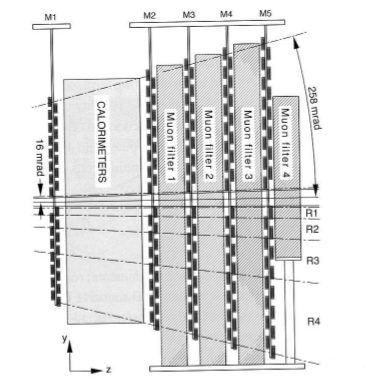
\includegraphics[width=0.5\linewidth]{Detector/figs/muonsystem.png}
\caption{The LHCb muon system \cite{Alves:2008zz}.}
\end{figure}

It is essential for many of the key physics analyses to be able to identify muons in the final state.
Muons are the most penetrating particles that can be detected at LHC experiments, so the muon chambers
are the final subdetectors. There are five stations (M1 - M5), the first one being located before the calorimeter
in order to improve the $p_T$ measurements. A scheme of the muon system is shown in Fig. \ref{muonsystem}.

The remaining four lay behind the HCAL and are separated by 1.2 m from each other, interleaved with iron block
filters 80cm thick, which absorb hadrons, electrons and photons to ensure that only muons reach the final muon station.
Only muons with a minimum momentum of 10 GeV/c traverse all of the five stations and for positive identification of a muon
the trigger requires a signal in each of them. Each station has a detection efficiency of at least 95\% and the detectors
provide position measurements. Since there is a larger particle flux towards the beam pipe, the stations are divided
into four concentric rectangular regions (R1-R4), their size increasing according to the ratio 1 : 2 : 4 : 8.
This means that there is a similar channel occupancy over the four regions. All of the muon stations use
Multi Wire Proportional Chambers (MWPC) except for the inner region of M1, where the particle flux is too high.
In this region triple-GEM (Gas Electron Multiplier) detectors are used instead because they have better ageing properties.

The Gas Electron Multiplier (GEM) detectors in the inner region of M1 have to  withstand a rate up to
$500 ~\mbox{kHz cm}^{-2}$ of charged particles. Particles traversing through the drift gap between the cathode
and the first GEM foil produce ionisation electrons which are then attracted by electric fields though all of the
GEM foils and they multiply. They then drift into the anode inducing a signal on the pads. A gas mixture of Argon,
$CO_2$ and $CF_4$, is used to give a time resolution better than 3 ns.




\subsection{Trigger and software}

The LHCb trigger system\cite{LHCb-DP-2012-004} consists of a hardware stage (L0), based on information from the calorimeter
and muon systems, followed by a software stage (HLT), which applies a full event reconstruction. To increase performances
the HLT is split again into stages (HLT1 and HLT2). The bunch crossing frequency is $40 ~\mbox{MHz}$, which corresponds
to an instantaneous luminosity of $2 \cdot 10^{32} ~\mbox{cm}^{-2} \mbox{s}^{-1}$ for LHCb, and about 15\% of the total
number of $b\bar{b}$ pairs produced will have at least one B meson with all of its decay products within the detector acceptance.
This needs to be reduced down to about 2 kHz so that the events can be written to disk for analysis. Fig. \ref{triggerscheme}
shows a scheme of the trigger system.

The L0 reduces the rate of visible interactions from 10 MHz to a rate of 1 MHz and uses mainly the information from the 
calorimeter dividing the events in the 5 categories: L0Photon, L0Electron, L0LocalPion, L0GlobalPion, L0Hadron. ``local" pions
refer to $\pi^0$ reconstructed though decay in $\gamma\gamma$, where the two photons fall in the same ECAL board, they are
labelled ``global" otherwise. The HLT1 uses information from the VELO and trackers performing a partial reconstruction
of the event and reduces the rate to 2 kHz. Finally the HLT2 involves a full reconstruction of the event and includes many
``lines" designed to trigger specific decays.

LHCb also developed an extended simulation software in order to reconstruct efficiencies and signal shapes.
In the simulation, $pp$ collisions are generated using $\textsc{Pythia}$~6.4\cite{Sjostrand:2006za} with a specific
LHCb configuration\cite{LHCb-PROC-2010-056}. Decays of hadronic particles are described by $\textsc{EvtGen}$\cite{Lange:2001uf},
in which final state radiation is generated using $\textsc{Photos}$\cite{Golonka:2005pn}. The interaction of the generated
particles with the detector and its response are implemented using the $\textsc{Geant4}$ toolkit\cite{Allison:2006ve, *Agostinelli:2002hh}
as described in \cite{LHCb-PROC-2011-006}.

For the analysis in this document, I used the ROOT framework\cite{Brun:2000es} to analyse data, the RooFit package
fot fitting. The multivariate analysis is base on ne NeuroBayes package \cite{} which provides a framework
for neural network training.

\begin{figure}[t!]
\label{triggerscheme}
\centering 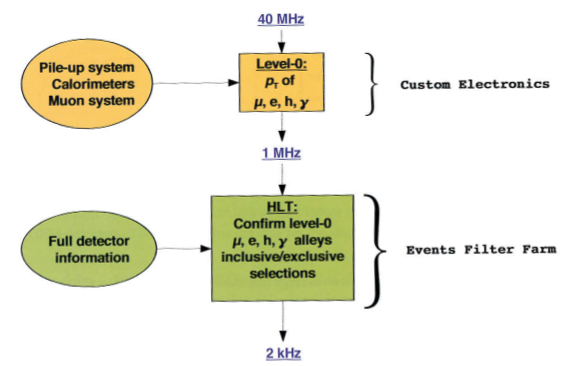
\includegraphics[width=0.8\linewidth]{Detector/figs/triggerscheme.png}
\caption{Scheme of the LHCb trigger system \cite{Alves:2008zz}.}
\end{figure}





